\documentclass[11pt]{article}
\usepackage[a4paper,margin=25mm]{geometry}
\usepackage{amsmath,amssymb,amsthm}
\usepackage{graphicx,booktabs}
\usepackage[pdfencoding=auto,hidelinks]{hyperref}
\DeclareMathSizes{10.95}{10.95}{8}{7}
\DeclareMathSizes{10}{10}{7}{7}
\DeclareMathSizes{9}{9}{7}{7}
\DeclareMathSizes{8}{8}{7}{7}
\graphicspath{{figures/}}
\hypersetup{pdftitle={Exactly two rational parity mixtures in quadratic Schwarzschild scattering},
pdfauthor={Aptifold Research},pdfsubject={Black-hole perturbation theory and machine-checked proofs}}
\newtheorem{theorem}{Theorem}
\newcommand{\ud}{\mathrm{d}}
\newcommand{\ii}{\mathrm{i}}
\newcommand{\EE}{\mathrm{EE}}
\newcommand{\EO}{\mathrm{EO}}
\newcommand{\OO}{\mathrm{OO}}

\title{Exactly two rational parity mixtures in\\quadratic Schwarzschild scattering}
\author{Aptifold Research\\[0.4em]
\small Research and formalization by the Aptifold AI system\\
\small Paul Wishall, human project lead}
\date{26 November 2026 \\ \small Preprint for technical review}

\begin{document}
\maketitle

\begin{abstract}
Consider two identical incident gravitational waves scattering from a Schwarzschild black hole in the maximal azimuthal channel
\((\ell,\ell)+(\ell,\ell)\to(2\ell,2\ell)\).
For every integer \(\ell\geq2\) and positive real common parent frequency, we classify the incident parity mixtures whose projected second-order equation admits a local quadratic particular solution with rational radial coefficients.
Exactly two mixtures have this property, one with a frequency-independent odd-to-even incident master ratio.
An exact obstruction rules out all other mixtures.
Pole and degree bounds reduce the exclusion to a \(41\times 30\) coefficient matrix.
A polynomial left-null witness excludes the source throughout the stated domain, and a Riccati argument extends coefficient matching to a single fixed nonzero parent wave.
Each particular solution gives a unique retarded completion. Its outgoing strain reduces to a boundary expression in linear reflection amplitudes.
Lean checks the projected source, completeness of the exclusion, rational and retarded uniqueness, and the readout of the physical strain.
The angular extension gives the solution across the entire top daughter for any azimuthal profile.
In a sensitive \(\ell=4\) case, two contributions each about \(48\) times larger than their sum cancel, and the fine integral agrees with the closed complex response within \(1.09\times10^{-20}\) in absolute normalized strain.
The second response has a change of sign in its first soft magnitude correction and a logarithmically drifting relative phase at the light ring.
\end{abstract}

\section{Introduction}

Suppose two incident gravitational waves have the same frequency \(\omega\) and angular label \(\ell\). Their interaction drives a new wave at \(2\omega\). We follow its highest angular daughter, \(L=2\ell\), on a Schwarzschild background.
The driving term depends on the first-order wave throughout the exterior.
An exact way to do the radial integral would turn a nonlinear waveform into a benchmark determined by linear scattering alone.

Aptifold asked which mixtures of the two incident parities permit this reduction. A rational local particular field is a quadratic expression in the parent wave and its radial derivative whose coefficients are rational functions of the areal radius. Such a field integrates the source locally. Imposing the boundary conditions then gives the physical response.

Regge--Wheeler and Zerilli theory supplies the parity-resolved linear operators \cite{reggewheeler,zerilli}, related by a Darboux transformation \cite{darboux}.
Bucciotti \emph{et al.} give the second-order scattering source, its regularization, the asymptotic strain normalization and the retarded Green integral used here \cite{bucciotti}. Their angular calculation supplies the mode weights, and their parity scan locates quadrupolar zeros of one spin component.
The locality criterion asks whether the source lies in the image of the daughter operator on a specified space of quadratic expressions.
Chen and Xie develop a general reduction of nonlinear Schwarzschild responses to master integrals \cite{chenxie}.
We classify the mixtures for which an explicit rational particular solution removes the radial integral in this channel. The classification is at real positive frequency. This distinguishes it from exact static response and the algebraically special sector at complex frequency \cite{iteanu,special}.

The second mixture supplies an additional test of physical response extraction.
It has both a term proportional to the square of the even parent reflection and a term proportional to the odd daughter reflection.
The two terms can nearly cancel.
This makes their complex relative phase and the sign of the incoming-wave subtraction directly testable.
Sections~\ref{sec:proof} and \ref{sec:strain} give the complete exclusion and the observable. Section~\ref{sec:lean} specifies the proof checked by Lean. Sections~\ref{sec:unique-retarded} and \ref{sec:followons} develop the retarded, angular, and frequency results.

\section{What Lean verifies}
\label{sec:lean}

The proof problem has three interfaces. The metric calculation supplies a
specific projected forcing. The rational operator acts on a proposed row
of local coefficients. The retarded solution satisfies boundary
conditions on a physical exterior wave. Lean checks the implications
between these interfaces as well as the finite arithmetic at the
center of the exclusion.

\begin{figure}[htbp]
 \centering
 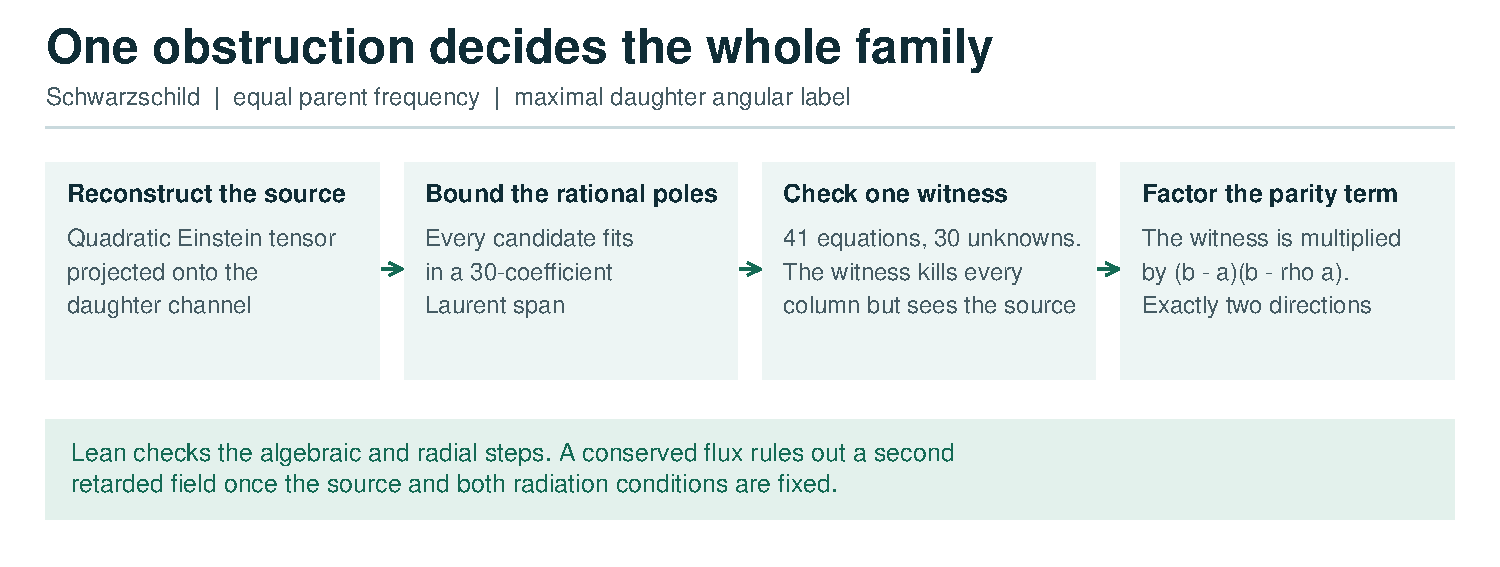
\includegraphics[width=\linewidth]{proof-chain.pdf}
 \caption{Structure of the classification argument. The 30 coefficients
 span all rational candidates after the pole and degree reductions.
 The witness is a linear functional of the 41 source equations. A
 nonzero witness projection proves that the source is outside the image
 of the operator.}
 \label{fig:proof-chain}
\end{figure}

\begin{description}
 \raggedright
 \item[Metric and source.] The checked coordinate and angular
 operations compute the quadratic Einstein tensor in the specified
 Schwarzschild perturbation ansatz. Separate reconstruction and
 conservation checks connect those components to the radial master
 source, including the relation to the pinned regularized source.
 \path{MetricMeromorphicClassification.lean} joins this chain to the
 local classification on a fixed nonzero parent germ.
 \item[All rational candidates.] The pole analysis at ordinary points,
 at the horizon and at zero, and the degree test at infinity reduce
 every possible row to the exhibited Laurent span.
 \path{MatrixCertificate.lean} checks the matrix columns and the
 source projection. The shifted coefficient sign proof covers every
 integer \(\ell\ge2\), and the exact parameter factors are nonzero at
 positive real frequency. The Riccati argument justifies coefficient
 matching even on a single parent solution.
 \item[Existence and uniqueness.] The checked source identities build
 a local row at each admitted ratio. \path{RationalLocalUniqueness.lean}
 rules out a nonzero rational homogeneous row.
 \path{LinearRetardedUniqueness.lean} proves the flux argument for the
 actual exterior boundary-value problem.
 \path{RetardedScattering.lean} constructs the two retarded fields and
 checks the printed strain formulas.
 \item[Extensions.]
 \path{AngularRetardedScattering.lean} proves existence and
 uniqueness for arbitrary azimuthal profiles in the top daughter.
 It combines two closed amplitudes with the pure-odd integral.
 Separate modules verify the angular obstruction, static comparison
 for the sharp-order absorption bound, the small-frequency magnitude
 sign calculation under the cited linear expansions, and the
 light-ring envelope transfer from its analytic matching hypotheses.
\end{description}

The guarded verification checked or hash-verified 1,208 modules in
the source and response development, with Lean 4.33.1 and a pinned
Mathlib revision. The named theorem checks require only the standard
Lean axioms \texttt{propext}, \texttt{Classical.choice} and
\texttt{Quot.sound}, or subsets. The public proof directory contains the
transitive source closure of the named results and lists the exact
toolchain and revision. It includes the algebraic polarization check
as a separately compiled extension.

Lean checks statements about the supplied equations and definitions.
The paper states the conventions that connect them to the physical
observables. The complex radial benchmarks and the fourth-multipole
zero enclosures use outward-rounded Arb arithmetic. The barrier-top
matching is an analytic argument, and the sign transfer explicitly
uses published linear expansion input. Related machine-checked
physics includes constructive field theory and local linear
Kerr--Newman perturbation equations \cite{douglas,wang}.


\section{Conventions and statement}
\label{sec:conventions}

We work in geometrized units and express radii and times in units of the Schwarzschild mass \(M\).
Thus the numerical frequency \(\omega\) below is the physical frequency multiplied by \(M\).
Set
\begin{equation}
 f=1-\frac{2}{r},\qquad
 x=r+2\log(r/2-1),\qquad
 D=\partial_x=f\,\partial_r,\qquad k=\ii\omega.
 \label{eq:conventions}
\end{equation}
We use time dependence \(e^{-\ii\omega t}\), so \(e^{-kx}\) travels toward the horizon and \(e^{kx}\) travels outward.
The additive constant in \(x\) is fixed by \eqref{eq:conventions}.
It matters for the complex phases.
For an angular index \(j\), define
\begin{align}
 \lambda_j&=\frac{(j-1)(j+2)}{2},
 &\gamma_j&=\frac{(j-1)j(j+1)(j+2)}{12},\\
 V_j&=f\left[\frac{j(j+1)}{r^2}-\frac{6}{r^3}\right],
 &W_j&=\gamma_j+\frac{3f}{r(\lambda_jr+3)} .
 \label{eq:parity}
\end{align}
Here \(V_j\) is the odd-parity potential.

Let \(E\) be the horizon-ingoing even parent at angular index \(\ell\), with its even incident amplitude set to one.
Use the reference odd master
\begin{equation}
 J=\frac{(W_\ell-D)E}{g-k},\qquad
 g=\gamma_\ell,\qquad L=2\ell,\qquad
 \Gamma=\frac{\gamma_L}{2},\qquad
 \alpha=\frac{g+k}{g-k}.
 \label{eq:darbourx}
\end{equation}
The incoming coefficient of \(J\) is \(\alpha\).
Its outgoing coefficient equals the even parent reflection amplitude.
An incident mixture has even parent \(aE\) and odd parent \(O=-\ii bJ\), with \((a,b)\ne(0,0)\).
For \(a\ne0\), \(\rho=b/a\) and the incident odd-to-even master ratio is \(p=-\ii\rho\alpha\).
The pure odd direction is included by using the homogeneous coordinates \([a:b]\).
Throughout we work with the complex channel coefficient of two identical parents. In particular, the selected daughter has \(m=L=2\ell\) and frequency \(2\omega\).

In the second-order regularization and strain convention of \cite{bucciotti}, write \(E_2,O_2\) for the daughter masters and define the projected variable
\begin{equation}
 X^-=\frac{(W_L-D)E_2}{\gamma_L-2k}-\ii O_2,\qquad
 \mathcal L_O=D^2-4k^2-V_L .
 \label{eq:daughter}
\end{equation}
In the algebra below we divide the field and source by the same common, nonzero angular projection factor, which is restored in section~\ref{sec:strain}.
The equation for the scaled field is
\begin{equation}
 \mathcal L_O X^-=S_{\mathrm{reg}}(a,b).
 \label{eq:forced}
\end{equation}
A rational local quadratic particular solution is a finite quadratic differential expression in the parent fields, with radial coefficients in \(\mathbb C(r)\) at fixed \(\ell\) and \(k\).
Each parent derivative can be reduced by the second-order parent equation and the parity map.
The admissible class is therefore the span over \(\mathbb C(r)\) of \(J^2,JZ,Z^2\), with \(Z=r^2DJ\).

\begin{theorem}
\label{thm:two}
For every integer \(\ell\geq2\) and every real \(\omega>0\), the projected equation \eqref{eq:forced} in the channel \((\ell,\ell)^2\to(2\ell,2\ell)\) admits a rational local quadratic particular solution exactly for
\begin{equation}
 [a:b]=[1:1]\quad\text{or}\quad[1:\rho_2],\qquad
 \rho_2=\frac{(\Gamma+g)(g-k)}{(\Gamma-g)(g+k)} .
 \label{eq:roots}
\end{equation}
The two solutions are regular on the ingoing parent at the future horizon, in the sense that their ingoing phase has a smooth radial envelope.
The corresponding incident odd-to-even master ratios are
\begin{equation}
 p_1=-\ii\,\frac{g+k}{g-k},\qquad
 p_2=-\ii\,\frac{\Gamma+g}{\Gamma-g}
     =-\ii\,\frac{9\ell^2+\ell-4}{7\ell^2-\ell}.
 \label{eq:masterratios}
\end{equation}
\end{theorem}

\section{Construction and exclusion}
\label{sec:proof}

\subsection{Construction at the two mixtures}

In the common odd reference basis, decompose the bare projected source into
\begin{equation}
 S(a,b)=a^2 S_{\EE}+ab S_{\EO}+b^2 S_{\OO},
 \label{eq:source}
\end{equation}
where \(S_{\EO}\) includes both mixed orderings.
The source polynomials are formed with the identical-parent normalization of \cite{bucciotti}.
The three regularizers of the referenced formulation add an image of \(\mathcal L_O\) on rational local fields.
They shift the particular solution by a known rational local field and leave membership in the same image invariant.

The exact coefficient calculations give rational fields \(P_1,P_\Delta\) obeying
\begin{align}
 \mathcal L_O P_1&=S(1,1),\\
 \mathcal L_O P_\Delta&=S_{\EO}+(1+\rho_2)S_{\OO}.
 \label{eq:construction}
\end{align}
The source and the solution coefficient rows are supplied with the algebraic certificate.
For either mixture the complete regularized projected source of \cite{bucciotti} is obtained from their even--even, mixed and odd--odd returns.
The symbolic comparison retains \(r,\ell,k\), the identical-parent factor and the regularizers.
For the odd--odd sector, let \(S^{\mathrm{pub}}_{\mathrm{bare}}\) denote the even daughter forcing obtained from the pinned published kernel by inserting \(J,J'\) in both parent slots, before the odd phase, the identical-parent half and removal of the angular factor.
The comparison verifies, coefficient by coefficient,
\[
 S_{\OO}=-\frac{1}{2\mathcal G_\ell}
     \frac{W_L-D}{\gamma_L-2k}\,S^{\mathrm{pub}}_{\mathrm{bare}},
 \qquad \mathcal G_\ell=C_\ell^2/C_L
\]
with \(\mathcal G_\ell\) specified in section~\ref{sec:strain}.
The two phases \(O=-\ii J\) give the minus sign, and the exchange-summed return for identical parents gives the factor \(1/2\).
Writing those rational additions as \(\mathcal U_{\EE},\mathcal U_{\EO},\mathcal U_{\OO}\), the field evaluated in the referenced regularization is
\begin{equation}
 \Pi_\rho=P_1+(\rho-1)P_\Delta+
    \mathcal U_{\EE}+\rho\mathcal U_{\EO}+\rho^2\mathcal U_{\OO},
 \quad \rho\in\{1,\rho_2\}.
 \label{eq:Pi}
\end{equation}
Substitution checks \(\mathcal L_O\Pi_\rho=S_{\mathrm{reg}}(1,\rho)\) in all three basis components.
For each \(\Pi_\rho=c_0J^2+c_1JZ+c_2Z^2\), the exact check first establishes that the three \(c_j\) have at most simple poles at \(r=2\), including after specialization anywhere in the stated parameter domain.
It then verifies the residue identity
\begin{equation}
 A-4kB+16k^2C=0,\qquad
 (A,B,C)=\left.(r-2)(c_0,c_1,c_2)\right|_{r=2}.
 \label{eq:horizon-cancel}
\end{equation}
On the ingoing parent \(Z/J=-4k+O(r-2)\). The residue identity therefore cancels the only possible pole in the ingoing envelope of \(\Pi_\rho\).

The residual of the general mixture factors as
\begin{equation}
 S(a,b)=\mathcal L_O\big[a^2P_1+a(b-a)P_\Delta\big]
       +(b-a)(b-\rho_2 a)S_{\OO}.
 \label{eq:factor}
\end{equation}
The roots are distinct. \(\Gamma-g=\ell^2(\ell+1)(7\ell-1)/12>0\), and the numerator of \(\rho_2-1\) in the common denominator is \(2(g^2-\Gamma k)\), with positive real part.
At \(a=0\) the residual coefficient is \(b^2\).
Thus it suffices to exclude one rational local image for the bare \(S_{\OO}\).
The regularized odd--odd source differs by the operator image already described.

\subsection{The finite operator test}

Put \(U=(J^2,JZ,Z^2)^{\mathsf T}\).
The odd parent equation is \(D^2J=(k^2+V_\ell)J\).
It gives \(DU=\mathsf B U\), where
\begin{equation}
 \mathsf B=
 \begin{pmatrix}
 0&2/r^2&0\\
 r^2(k^2+V_\ell)&2f/r&1/r^2\\
 0&2r^2(k^2+V_\ell)&4f/r
 \end{pmatrix}.
 \label{eq:jet}
\end{equation}
For a coefficient row \(c\), define \(\mathcal D c=Dc+c\mathsf B\).
The operator on rows is
\begin{equation}
 \mathcal L_O(cU)
 =\big[\mathcal D^2c-(4k^2+V_L)c\big]U .
 \label{eq:rowop}
\end{equation}
Appendix~\ref{app:independence} shows that this coefficient description remains faithful for a fixed nonzero parent, including the horizon-ingoing solution.

The audited bare \(S_{\OO}\) has pole orders \(6,0,3\) in each component at \(r=0,2,r_d\), respectively, with \(r_d=-3/\lambda_L\).
Its Laurent remainder after subtracting the forced nonzero-radius pole image has degree at most three in the unscaled basis \((J,DJ)\).
Appendix~\ref{app:poles} gives the pole and degree bounds.
After subtracting the forced simple principal part at \(r_d\), a rational candidate has at most a seventh-order pole at the origin, no other finite poles, and maximum degrees \(4,2,0\) in the three components of \(c\).
The allowed powers are therefore
\begin{equation}
  [-7,4],\qquad [-7,2],\qquad [-7,0],
 \label{eq:cols}
\end{equation}
giving 30 unknowns.
The powers of the output rows are \([-11,4]\), \([-11,1]\), \([-11,0]\), giving 41 equations.
Let \(H\) be this \(41\times30\) Laurent matrix for \eqref{eq:rowop}, with \(s\) the source remainder in the same row order.

A saved polynomial row \(w\) satisfies
\begin{equation}
 wH=0,\qquad ws=\frac{k^6 A(\ell)}{k-\Gamma},
 \label{eq:witness}
\end{equation}
where \(A\in\mathbb Q[\ell]\) has degree 65.
The calculation reconstructs every operator column and verifies \eqref{eq:witness} by exact polynomial arithmetic.
For the angular factor, exact evaluation gives \(A(j)\ne0\) for \(j=2,\ldots,17\).
All coefficients of \(A(18+t)\) are nonnegative and the constant coefficient is positive, so the factor is positive for \(\ell\geq18\).
The denominator and \(k^6\) are nonzero on the stated frequency domain.
Thus \(ws\ne0\), independently of the rank of \(H\) after specialization, and the Laurent linear system has no solution.
Together with \eqref{eq:factor} this proves Theorem~\ref{thm:two}.
The coefficient matrix, witness and exact check are available with the \hyperref[sec:data]{data and code}.

\section{Closed physical response}
\label{sec:strain}

Define \(R_p=R_{\ell,E}(\omega)\) and \(R_d=R_{L,O}(2\omega)\) as outgoing over incoming linear master amplitudes of the horizon-ingoing solutions, using the same origin of \(x\).
For the spin-weight \(-2\) harmonic normalized as in \cite{bucciotti}, the master-to-strain factor is \(N_j=\sqrt{(j+2)!/(j-2)!}/2\).
The outgoing strain combines \(E-\ii O\), and the incoming strain combines \(E+\ii O\).
For unit even incidence at mixture \(\rho\), the incoming parent strain amplitude, after removing the radial \(1/r\) factor, is \(N_\ell(1+\rho\alpha)\).
Our \(Q^-_{\rho,\ell}\) is the outgoing daughter amplitude divided by the square of that incoming parent amplitude in the \(M=1\) units of section~\ref{sec:conventions}.
With \(M\) restored this is the dimensionless incoming normalization in Eq.~(27) of \cite{bucciotti}.
In the first mixture the outgoing \emph{linear parent} spin-minus amplitude vanishes, since it is \(N_\ell(1-\rho) R_p\).
The incoming normalization is nonzero. The factor \(1+\rho\alpha\) equals \(2g/(g-k)\) for the first mixture and \(2\Gamma/(\Gamma-g)\) for the second.

For each of the two local fields \(\Pi_\rho\), let \(u\) be the horizon-ingoing odd homogeneous daughter.
The Green integral in Eq.~(32) of \cite{bucciotti} becomes a boundary term.
\begin{equation}
 uS_{\mathrm{reg}}=u\mathcal L_O\Pi_\rho
 =D(uD\Pi_\rho-\Pi_\rho Du).
 \label{eq:current}
\end{equation}
The horizon current vanishes because both fields have the same ingoing carrier and smooth envelopes.
The two signed sectors of \(\Pi_\rho\) at infinity have finite leading coefficients \(b_{++}\) and \(b_{--}\), normalized on unit outgoing or incoming reference-parent waves, respectively.
The mixed sector is \(O(r^{-2})\).
These coefficients follow by expanding the exact rational fields using
\begin{equation}
 J_\sigma=e^{\sigma kx}F_\sigma(r),\quad
 F_\sigma=1+O(r^{-1}),\qquad
 D^2F_\sigma+2\sigma k DF_\sigma-V_\ell F_\sigma=0,\quad \sigma=\pm1 .
 \label{eq:asymptotic}
\end{equation}
Substitution of a series in \(1/r\) into \eqref{eq:asymptotic} fixes the needed terms in each sector.
For \(u\sim A_{\mathrm{in},d}e^{-2kx}+A_{\mathrm{out},d}e^{2kx}\), division of the current by \(4k A_{\mathrm{in},d}\) yields
\begin{equation}
  b_{++} R_p^2-\alpha^2 b_{--}R_d .
 \label{eq:endpoint}
\end{equation}
At infinity the Darboux map in \eqref{eq:daughter} preserves an outgoing even daughter amplitude and multiplies an incoming even daughter amplitude by \((\Gamma+k)/(\Gamma-k)\).
Zero incoming amplitude in each daughter parity master therefore implies zero incoming amplitude in \(X^-\).
The local \(\Pi_\rho\) has incoming coefficient \(\alpha^2 b_{--}\) in the scaled projected master. Subtracting \(\alpha^2 b_{--}\,u/A_{\mathrm{in},d}\) imposes the derived projected boundary condition and gives the sign in \eqref{eq:endpoint}.
The conserved real-frequency flux of \(u\) implies \(A_{\mathrm{in},d}\ne0\).

Restore the angular projection factor \(\mathcal G_\ell=C_\ell^2/C_L\) with
\(C_j^2=(2j+1)!/[4\pi\,2^{2j}(j!)^2]\)
in the maximal-\(m\) scalar harmonic convention \cite{bucciotti}.
The multiplicative conversion of \eqref{eq:endpoint} is then
\(B_\ell/(1+\rho\alpha)^2\), where \(B_\ell=N_L\mathcal G_\ell/N_\ell^2\).
Evaluation of the endpoint coefficients gives
\begin{align}
 Q^-_{1,\ell}
   &=\frac{K_\ell k^2}{4g^2(k-\Gamma)}R_d ,
 \label{eq:Qone}\\
 Q^-_{2,\ell}
   &=\frac{K_\ell}{4\Gamma}\left[
        \frac{k(k-g^2/\Gamma)}{(k+g)^2}R_p^2
       +\frac{k}{k-\Gamma}R_d
     \right] ,
 \label{eq:Qtwo}\\
 K_\ell
   &=\frac{(2\ell+1)!(20\ell^3+35\ell^2+\ell-8)}
           {144(\ell-1)!(\ell-2)!}
     \sqrt{\frac{(2\ell+2)!(2\ell-2)!}{\pi(4\ell+1)!}} .
 \label{eq:K}
\end{align}
Here the subscripts 1 and 2 refer to \eqref{eq:roots}.
One check on the angular normalization is the rational quotient
\begin{equation}
 \frac{K_\ell}{B_\ell}
 =\frac{(20\ell^3+35\ell^2+\ell-8)\ell^2(\ell-1)^2(\ell+1)(\ell+2)}
        {288(2\ell-1)} .
 \label{eq:KoverB}
\end{equation}
Equations~\eqref{eq:current}--\eqref{eq:K} evaluate the previously published Green integral in these two cases, in its stated source and physical strain convention.
They give the complex phase as well as the magnitude.

\section{Radial benchmarks}
\label{sec:numerics}

We tested \eqref{eq:Qone} and \eqref{eq:Qtwo} by direct radial source integrations at the parameter points in table~\ref{tab:bench}.
The \(\ell=2,3\) comparisons use separately constructed native source and gauge expressions, with common admitted linear waves.
The \(\ell=4\) calculation specializes the pinned published regularized source, propagates the horizon-ingoing linear waves and integrates the source without evaluating the closed-response formula.
The subsequent comparison uses the linear reflection estimates from that same wave propagation.
It tests the second-order integration, boundary subtraction and complex phase for common input waves.

\begin{table}[htbp]
 \centering
 \small
 \begin{tabular}{ccclc}
 \toprule
 \(\ell\)&\(\omega\)&Mixture&\(Q^-\) (rounded)&Absolute difference bound\\
 \midrule
 \(2\)&\(3/8\)&1&\(-0.00415795823-0.00240124858\ii\)&\(1.24\times10^{-28}\)\\
 \(2\)&\(3/8\)&2&\(0.00092441138+0.00123941329\ii\)&\(6.25\times10^{-29}\)\\
 \(3\)&\(1/4\)&1&\((2.11266445+0.99492748\ii)\,10^{-4}\)&\(1.008\times10^{-25}\)\\
 \(3\)&\(1/4\)&2&\((1.71049373+2.92249500\ii)\,10^{-5}\)&\(1.507\times10^{-25}\)\\
 \(4\)&\(1/2\)&2&\((3.17716650+1.47588700\ii)\,10^{-5}\)&\(1.09\times10^{-20}\)\\
 \bottomrule
 \end{tabular}
 \caption{Complex strain checks in units \(M=1\).
 The last column bounds \(\lvert Q^-_{\rm direct}-Q^-_{\rm closed}\rvert\) using the calculation enclosures. The displayed central values are rounded separately. The quadrupole bounds
are rounded upward from the archived enclosures supplied with the supplement.}
 \label{tab:bench}
\end{table}

At \(\ell=4,\ \omega=1/2\), the two terms in \eqref{eq:Qtwo} have magnitudes approximately \(1.68194\times10^{-3}\) and \(1.67109\times10^{-3}\), while their sum has magnitude \(3.50323\times10^{-5}\).
Figure~\ref{fig:cancel} shows the contributions in the complex plane.
The two radial resolutions use horizon offsets \(1/128\) and \(1/256\), outer radii 128 and 176, and 1575 and 2006 finite panels.
They give overlapping enclosures.
The complex enclosures bound \(\lvert Q^-_{\rm direct}-Q^-_{\rm closed}\rvert\) by \(1.32\times10^{-14}\) and \(1.09\times10^{-20}\) respectively, for the shared input waves at this benchmark.
Omitting either reflection term or reversing one sign misses the fine enclosure by more than \(1.67\times10^{-3}\).

\begin{figure}[htbp]
 \centering
 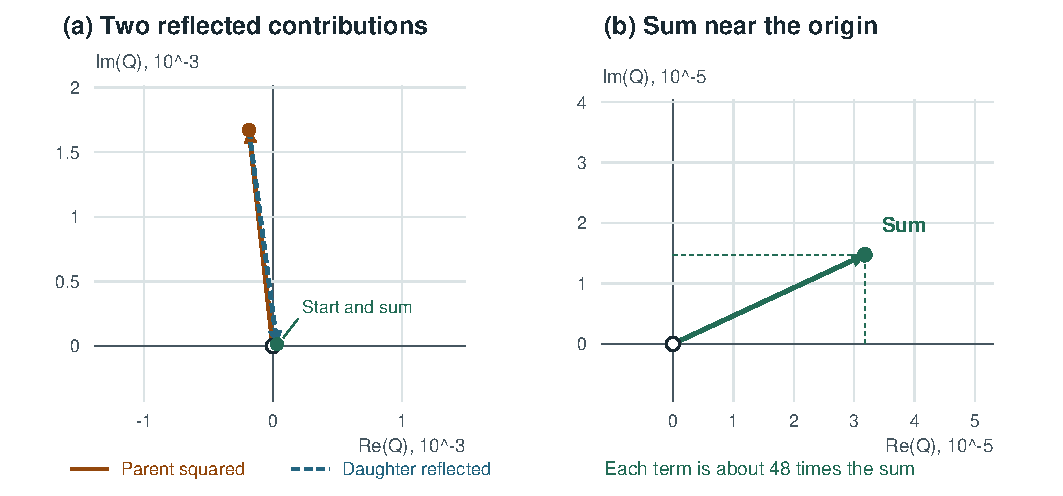
\includegraphics[width=\linewidth]{cancellation.pdf}
 \caption{Cancellation at \(\ell=4,\ \omega=1/2\) for the second mixture.
 (a) The parent-squared and daughter-reflection contributions are drawn head to tail.
 (b) Magnified view of their sum.
 Both coordinates in each panel use the same scale. The symbols mark the start, intermediate point and resultant.}
 \label{fig:cancel}
\end{figure}

The direct radial calculation integrates the compiled source against the horizon-ingoing homogeneous daughter.
At the horizon it uses the exact ingoing carrier and a convergent power series for the envelope.
On the finite interval, Cauchy bounds control the truncated panel integrals.
For a linear wave of frequency \(\nu\) the propagation norm is that of \((y,Dy/\nu)\), using \(\nu=\omega\) for the parent and \(\nu=2\omega\) for the daughter. The free part is skew-Hermitian and the potential controls the growth budget.
The infinity treatment includes the resonant and nonresonant phases, with remainder bounds on both the wave expansion and the integration.
A manufactured local field tests the endpoint contributions independently of the two physical responses.
The ancillary radial archive contains both direct enclosures and their comparison with \eqref{eq:Qtwo}.

\paragraph{Cross-check of the infinity contribution.}
The oscillatory far-tail remainder dominates the fine integration error budget.
A separate quadrature uses the same pinned radial kernels and linear amplitudes, evaluates the rational kernels directly, and treats the two zero-phase branches in \(t=1/r\).
For each nonzero phase \(q\), it deforms the polynomial Jost approximation to \(r=176+\ii\,\operatorname{sgn}(q)s\).
In the deformation region \({\rm Re}(r)\ge 176\) the denominators are nonzero, the logarithm has a continuous branch, and the phase magnitude on the ray is bounded by \(e^{-|q|s}\).
A separate real-axis Volterra bound controls the error of replacing the Jost waves by their polynomials.
The resulting normalized tail enclosure is contained in the original fine enclosure.
Omitting the \(q=+2\) branch gives a disjoint enclosure with a difference exceeding \(8.04\times10^{-7}\).
The referee supplement includes both numerical routes.

\paragraph{Check of the linear reflection inputs.}
A second linear solver computes the even parent directly with the Zerilli potential and the odd daughter with the Regge--Wheeler potential.
It uses extrapolated modified midpoint propagation in \(r\) with independently constructed endpoint series and 192-bit arithmetic.
Three resolutions vary the horizon offset, matching radius and propagation step.
The two finest results change either complex reflection by less than \(2.5\times10^{-23}\).
With the fixed phase origin, inserting these reflections in \eqref{eq:Qtwo} changes the archived closed comparison by less than \(8\times10^{-25}\) in normalized strain.
This convergence check exercises the shared linear inputs to the direct and closed calculations.

\section{The unique retarded field}
\label{sec:unique-retarded}

A local particular solution is a way to integrate the source at each radius.
The physical boundary conditions are separate. They require the daughter to
propagate into the future horizon and out to infinity, with no incoming
daughter from infinity. We impose these mode limits on the field and its
tortoise derivative. The constants in the incoming parent wave remain fixed.

Let \(u\) be the homogeneous daughter with unit ingoing amplitude at the
horizon, and let \(A_{\mathrm{in}},A_{\mathrm{out}}\) be its amplitudes at
infinity. Write \(w=2k\). At the real physical frequency, the conserved
Wronskian \(W_D(u,\overline u)=2w\) implies
\[
 |A_{\mathrm{in}}|^2-|A_{\mathrm{out}}|^2=1 .
\]
The difference of two solutions with the same source solves the homogeneous
equation. In the basis \(u,\overline u\), the absence of an outgoing horizon
mode forces that difference to equal \(c u\). The absence of an incoming
infinity mode gives \(c A_{\mathrm{in}}=0\). The flux identity makes
\(A_{\mathrm{in}}\) nonzero, so \(c=0\).
This is an exterior uniqueness result at nonzero real frequency. It holds
for any forcing for which a solution has the stated radiation limits.

For each admitted mixture, the regular local field provides one particular
solution. If its incoming coefficient in the scaled projected master is
\(\alpha^2 b_{--}\), subtracting \(\alpha^2 b_{--}u/A_{\mathrm{in}}\)
produces the unique retarded field. This proves the wave solution and the
sign of the subtraction in the boundary expression. The absence of a
homogeneous \emph{rational row} is a second result, at the level of local
coefficients. Its zero-source Laurent bounds leave 18 columns. A nonzero
minor is proportional to
\[
 \ell(3\ell+1)\,[1008 k^2-P(\ell)].
\]
The angular factor is
\[
 \begin{aligned}
 P(\ell)={}&259\ell^8+524\ell^7+134\ell^6-280\ell^5\\
           &-133\ell^4+44\ell^3+28\ell^2 .
 \end{aligned}
\]
Every coefficient of \(P(2+x)\) is positive, and \(k^2<0\).
Consequently each admitted rational row is unique.

\subsection{A Green solution for an arbitrary incident profile}

The classification does not prevent the field for another incident
polarization from having a retarded response. Define
\[
 v=\overline u-\frac{\overline A_{\mathrm{out}}}{A_{\mathrm{in}}}u .
\]
At infinity \(v\) is outgoing, with amplitude \(1/A_{\mathrm{in}}\).
Its Wronskian with \(u\) is \(2w\). For a source \(S\) such that both
integrands are absolutely integrable, the retarded field is
\[
 X_{\rm ret}(r)=\frac{1}{2w}
   \left[
       v(r)\int_2^r \frac{u(s)S(s)}{f(s)}\,\ud s+
       u(r)\int_r^\infty \frac{v(s)S(s)}{f(s)}\,\ud s
   \right].
\]
Differentiation cancels the two moving endpoints in the first derivative,
and the Wronskian produces \(S\) in the second. The same absolute
integrability proves the horizon and infinity mode limits for the field
and its jet. The pure-odd source meets the hypothesis because the ingoing
contraction vanishes at \(r=2\), with \(S/f=O(1)\), and its unscaled radial
coefficients are \(O(r^{-2})\) at infinity. The source and both homogeneous
waves remain bounded after the respective endpoint scalings. The pure-odd
amplitude is a single absolutely convergent integral \(\int_2^\infty
uS/f\) divided by \(2w A_{\mathrm{in}}\).
The two admitted responses and this third response span the full quadratic
dependence on the incident parity coefficients.

\subsection{All azimuthal components of the highest daughter}
\label{sec:angular-followon}

Let \(N=2\ell\), and use even and odd incident polynomials
\[
 A(z)=\sum_{p=0}^N \sqrt{\binom{N}{p}}\,a_{\ell-p} z^p,\qquad
 B(z)=\sum_{p=0}^N \sqrt{\binom{N}{p}}\,b_{\ell-p} z^p.
\]
For the top daughter the Clebsch--Gordan product weight is
\(\sqrt{\binom{N}{p}\binom{N}{q}/\binom{2N}{p+q}}\).
This is the maximal-coupling specialization of the radial and angular
separation in \cite[Sec.~V.4]{bucciotti}. The coefficient of \(z^s\) is
the daughter with \(m=2\ell-s\), after division by the nonzero factor
\(\sqrt{\binom{2N}{s}}\).

The rational obstruction for that daughter is proportional to
\([z^s](B-A)(B-\rho_2 A)\), with \(\rho_2\) from
Theorem~\ref{thm:two}. The whole top multiplet has rational local rows
if and only if \(B=A\) or \(B=\rho_2 A\), because
\(\mathbb{C}[z]\) has no zero divisors.
Even two parent modes that each lie on an admitted branch can create
a cross mode without a rational row. If \(A=z^p+z^q\) and
\(B=z^p+\rho_2 z^q\), the obstruction is
\(-(\rho_2-1)^2z^{p+q}\).

For arbitrary \(A,B\) let
\[
 D(z)=\frac{A(B-A)}{\rho_2-1},\qquad
 C(z)=(B-A)(B-\rho_2 A).
\]
If \(q_1,q_2\) are the common-basis outgoing coefficients of the admitted
mixtures and \(q_{\rm O}\) is the pure-odd integral above, the outgoing
component is
\[
 [z^s]\big((A^2-D)q_1 + Dq_2 + Cq_{\rm O}\big)
\]
with the same angular division. This formula follows by expanding the
three source rows in the common parent basis and using linearity and
uniqueness of the daughter solution.

\section{What the exact responses reveal}
\label{sec:followons}

\subsection{A sign switch in the first low-frequency correction}

The published simulations find leading quadratic scaling in \(M\omega\)
for the studied channels \cite{bucciotti}. Our local formulas make the
first branch-dependent correction accessible.
For the second mixture, the first correction to the leading
frequency-squared-normalized magnitude is negative at \(\ell=2,3,4\) and
positive at every integer \(\ell\ge5\). With \(j\) an angular label the
signed factor is \(d_\ell-2d_{2\ell}\), where
\[
 d_j=\frac{1}{2j+1}
   \left[-2-\frac{4}{j(j+1)}
     +\frac{[(j+1)^2-4]^2}{(2j+1)(2j+2)(2j+3)}
     -\frac{(j^2-4)^2}{(2j-1)(2j)(2j+1)}
   \right].
\]
The linear expansion uses the low-frequency phase and renormalized
angular momentum of \cite{dolan,mst}. The common unit phase cancels from
the magnitude. The positive threshold factor and the sign of the
remaining angular polynomial are separately checked in Lean.
Figure~\ref{fig:soft-sign} supplies two finite-frequency witnesses.
The sign calculation uses the cited linear expansions as premises.
If \(\sigma_\ell\) denotes this slope after division by the leading
coefficient as well as \((M\omega)^2\), then
\(\ell\,\sigma_\ell\to15\pi/16\) in that expansion.

The condition for cancellation of the second admitted strain is more
restrictive at small positive frequency. From the two prefactors,
\[
 Q^-_2=P(k)\big(C(k)R_p^2+R_d\big),\quad
 C(k)=1-\chi+\chi\left(\frac{k-g}{k+g}\right)^2,\quad
 \chi=\frac{(G+g)^2}{4Gg},
\]
where \(g=\gamma_\ell\), \(G=\gamma_{2\ell}/2\), and
\(P(k)=K_\ell k/[4G(k-G)]\) is nonzero.
The squared quotient has unit modulus, so \(C(k)\) traces a circle.
Its modulus exceeds one by a positive quadratic correction near zero.
The loss \(1-|R_p|^2\) is bounded by \(O_\ell((M\omega)^{2\ell+2})\)
using a static positive barrier comparison, consistent with the
published leading absorption law \cite{grayvisser}. Since
\(|R_d|\le1\), the triangle inequality yields
\(|Q^-_2|\ge c_\ell (M\omega)^3>0\) for sufficiently small positive
frequency at every fixed \(\ell\).

\begin{figure}[htbp]
 \centering
 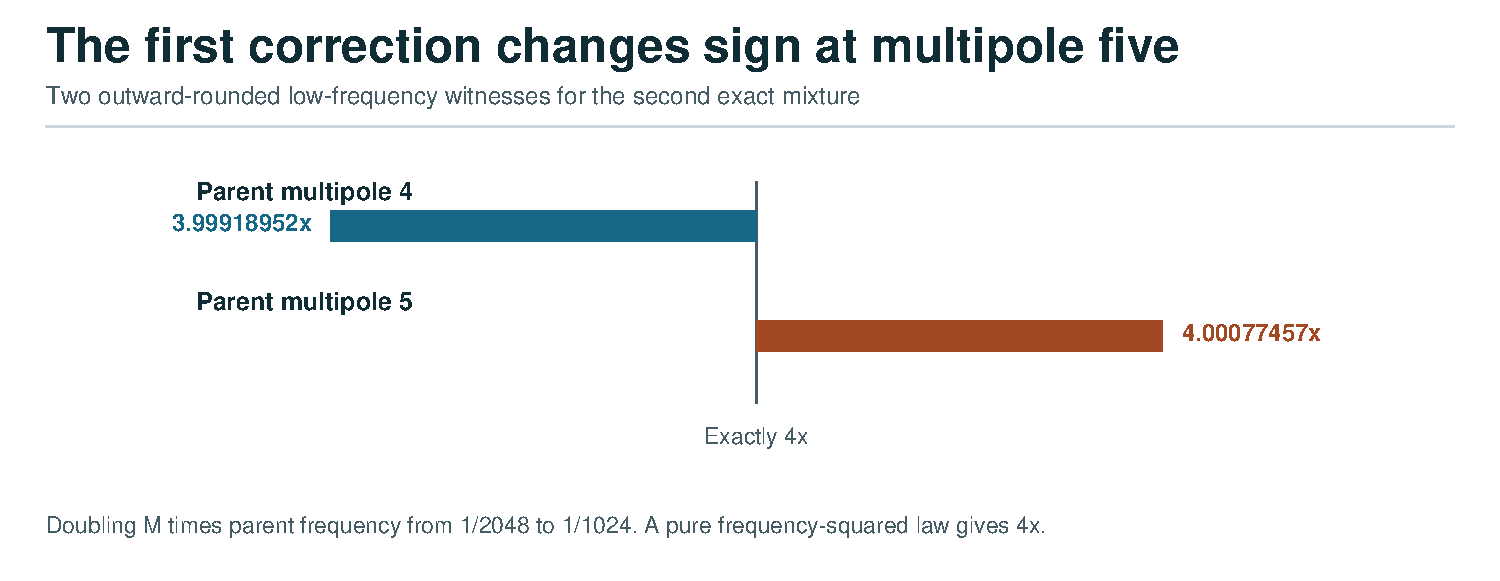
\includegraphics[width=\linewidth]{soft-sign.pdf}
 \caption{A finite-frequency check of the first correction to quadratic
 growth. The second-mixture amplitudes use the incoming-strain convention
 of Section~\ref{sec:strain}. The plotted doubling ratios are rounded
 from outward enclosures. The general sign statement is asymptotic.}
 \label{fig:soft-sign}
\end{figure}

\subsection{A resolved interference dip and two polarization zeros}

At \(\ell=4\) on \(0.650\le M\omega\le 0.675\), interval propagation and
frequency interpolation bound the second admitted response away from
zero on the entire band. Every minimum over that band lies in
\(0.66219<M\omega<0.66565\), with magnitude between
\(1.2130\times10^{-5}\) and \(1.2247\times10^{-5}\).
Exact phase opposition occurs at a lower frequency in
\([0.655,0.660]\), where the two term magnitudes differ by a factor
of at least \(1.00234\). The minimum of the strain magnitude need not
coincide with the crossing of the relative phase.

One may instead change the incident polarization. At the fixed
\(\ell=4,\ M\omega=1/2\) benchmark, write the spin-minus amplitude in
the common parent basis as
\[
 P_-(a,b)=E a^2+Xab+O b^2 .
\]
\begin{figure}[htbp]
 \centering
 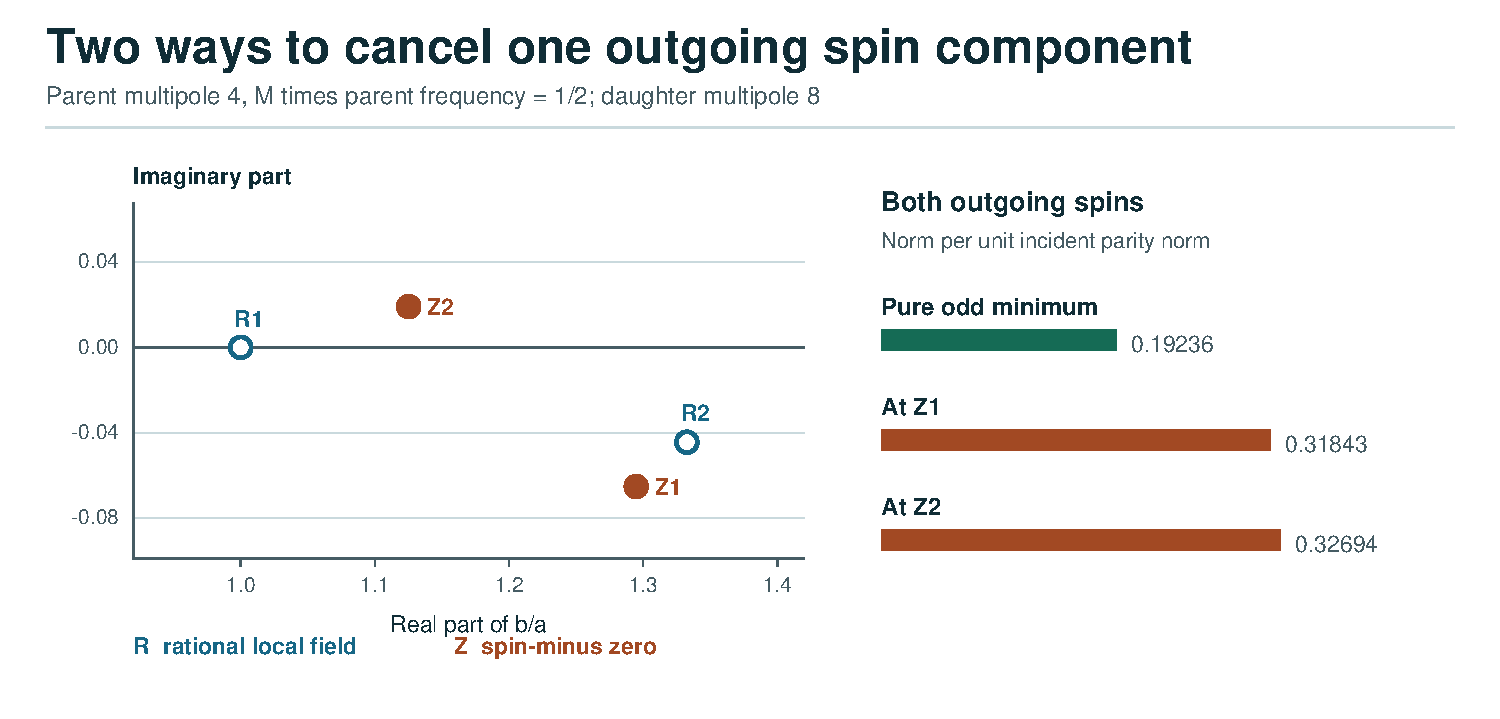
\includegraphics[width=\linewidth]{polarization.pdf}
 \caption{The two rational ratios \(R1,R2\) and the two outgoing
 spin-minus zeros \(Z1,Z2\) are disjoint at the benchmark. The bars
 show the norm of the two outgoing spin amplitudes at fixed unit
 incident parity norm in the common parent basis.}
 \label{fig:polarization}
\end{figure}
We integrate each source component separately on two grids
using the pinned regularized source. Adding the components recovers
both admitted amplitudes and a manufactured source recovers the exact
currents on the horizon, finite interval and infinity pieces.
Direct ball arithmetic isolates two simple roots,
\[
 b/a\simeq 1.294793416343-0.065231726339\,\ii,\qquad
 b/a\simeq 1.125230638044+0.019148752108\,\ii.
\]
Their incident strain normalization is nonzero. Each differs from both
admitted rational ratios. Prior work already found two nearby zeros
under quadrupolar driving \cite[Sec.~V.5, Fig.~6]{bucciotti}. The
result here certifies this fourth-multipole example, links it to the
different rational-local condition, and extends the zero criterion to
all azimuthal modes.

For a general angular profile, \(\mathbb{C}[z]\) has no zero divisors.
The entire top daughter has vanishing spin-minus amplitude exactly when
\(B=\zeta_1 A\) or \(B=\zeta_2 A\), where \(\zeta_i\) are the two roots.
Parity flips only the mixed term for the opposite spin component.
Hence simultaneous vanishing of the two output polynomials would give
\(XAB=0\) and \(EA^2+OB^2=0\). At the benchmark all three coefficients
are nonzero. The only joint zero is zero incident data.
For one incident mode, the half squared output norm is
\[
 |Ea^2+Ob^2|^2+|X|^2 |ab|^2 .
\]
Set \(e=|E|,x=|X|,o=|O|\) and \(t=|a|^2\) with
\(|a|^2+|b|^2=1\). The reverse triangle inequality bounds this by
\(o^2+t[(1-t)(x^2-2o(o+e))+t(e^2-o^2)]\) from below. Both
coefficients inside the brackets are strictly positive in the interval
calculation, so pure odd incidence attains the minimum. Figure~\ref{fig:polarization}
shows that either spin-minus zero leaves a larger total two-spin norm.
The lower bound also gives a floor for arbitrary unit incident profiles.
In the binomial normalization, the squared norm of a polynomial \(P\)
of degree at most \(D\) is
\((D+1)\int |P(z)|^2/(1+|z|^2)^D\,\ud\mu\), with \(\mu\) the
normalized sphere measure. Apply the pointwise scalar lower bound
before integrating and use Jensen's inequality. The daughter norm
is at least \(\sqrt{2(2N+1)}\,o/(N+1)\), about \(0.08812\) in the
common units for \(N=8\). This holds for every unit angular profile,
including profiles with unrelated phases in their two parities.

\subsection{A logarithmically drifting phase at the light ring}

Fix real detuning \(\delta\), with the daughter frequency chosen as
\(2M\omega=(2\ell+\delta)/(3\sqrt3)\), and let \(\ell\) run through
positive integers. Write
\[
 F(b)=\big(1+e^{\pi(2b-1)}\big)^{-1},\quad
 K_0=\frac{5\,2^{1/4}}{36\pi^{3/4}},\quad C_2=\frac{\sqrt3 K_0}{16}.
\]
The first mixture has
\(\ell^{15/4}|Q^-_{1,\ell}|\to 2K_0\sqrt{F(\delta)}\).
The second has a lower and an upper limiting envelope,
\[
 \begin{split}
 \liminf_{\ell\to\infty}\ell^{3/4}|Q^-_{2,\ell}|
   &= C_2\,|F(\delta/2)-\sqrt{F(\delta)}|,\\
 \limsup_{\ell\to\infty}\ell^{3/4}|Q^-_{2,\ell}|
   &= C_2\,[F(\delta/2)+\sqrt{F(\delta)}].
 \end{split}
\]
The two contributions settle in modulus on this scale while their
relative phase keeps changing. Its leading form is
\(\tfrac12\log\ell+\theta(\delta)+o(1)\) modulo \(2\pi\).
It is invariant under translation of the tortoise-coordinate origin
because the frequencies add exactly.

The matching uses the Weber barrier-top connection, as in the linear
semiclassical problem \cite{ramond,dlmf}. Specifically let
\(h=(j+1/2)^{-1}\) for an individual linear wave and use
\(M w_{\rm lin}=(j+b)/(3\sqrt3)\).
Near \(r=3\), \(V_0=f/r^2\) has a nondegenerate maximum
\(a=1/27\) in the \(M=1\) convention. After the scaling \(x=\sqrt h\,y\)
the leading equation is
\[
 U''+(a^2 y^2+2a(b-1/2))\,U=0 .
\]
Matching at \(x=\pm h^{2/5}\) gives a coefficient error
\(O(h^{1/5})\) at fixed detuning. The inner remainder integrates as
\(O(\sqrt h Y^3+h\log(1+Y))\) with \(Y=h^{-1/10}\) in the Weber
basis. On the exterior the WKB error is controlled by
\(O(h\,h^{-4/5})\) at the cut and by integrable tails. The
linear phase includes \((b-1/2)\log(j+1/2)\).
In \(R_d/R_p^2\), its logarithmic coefficient is
\((\delta-1/2)-2(\delta/2-1/2)=1/2\).
The global action terms leave a constant, and the parent Darboux
phase tends to one. The full matching, including the exterior
phase constants, is supplied with the source.

\begin{figure}[htbp]
 \centering
 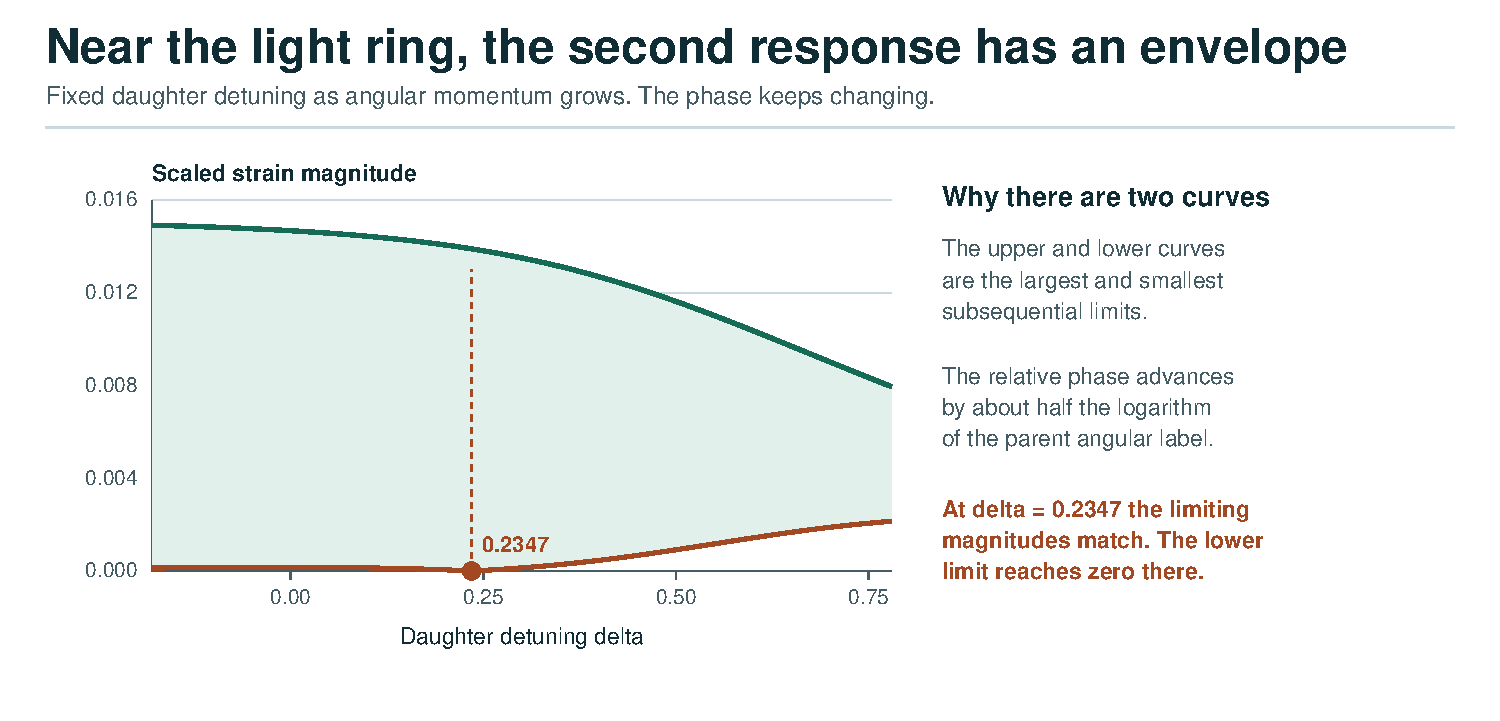
\includegraphics[width=\linewidth]{light-ring.pdf}
 \caption{The second-mixture light-ring limits. Fixed detuning
 \(\delta\) is measured relative to the leading daughter frequency.
 The lower limit reaches zero only at the limiting magnitude
 balance. It is attained along subsequences with increasing \(\ell\).}
 \label{fig:light-ring}
\end{figure}

Integer labels nearest to
\(\exp(2(2\pi m+\varphi-\theta))\) realize any relative phase
\(\varphi\) in the limit. This gives both envelopes. They balance at
\(\delta_\ast = 1+\pi^{-1}\log(2/(e^\pi-1))\simeq0.23469708\),
where a subsequence of the scaled magnitude approaches zero. The
statement concerns the limit, and leaves open exact finite-label zeros
along these two admitted branches and the separate pure-even eikonal
question of \cite[Sec.~V.3]{bucciotti}.
Lean checks the envelope and phase-subsequence argument from the
linear matching hypotheses. Numerical controls use different
propagators and extraction methods to check the analytic phase.


\section{Scope and implications}

The classification concerns the existence of a rational local particular field for the selected second-order source.
The strain-zero condition studied in \cite{bucciotti} concerns the value of the response after physical boundary completion.
For example, both mixtures in Theorem~\ref{thm:two} radiate nonzero spin-minus daughter strain at the quadrupole benchmark in table~\ref{tab:bench}, with magnitudes about \(0.00480\) and \(0.00155\).
The earlier calculation supplies the source, strain map and retarded completion. The locality result fixes the two incident directions where that evaluation reduces to boundary terms.
Likewise, the general integration-by-parts construction of \cite{chenxie} supplies the reduction framework. Here the finite obstruction decides exactly which parity mixtures allow a rational local identity in this angular family.

The proof uses integer angular labels, common real positive frequency and the maximal azimuthal channel at second order on Schwarzschild.
The algebraically special imaginary-frequency case in appendix~\ref{app:independence} illustrates why the frequency condition enters the fixed-parent argument.
Related exact second-order results in the algebraically special sector use that distinct frequency and boundary regime~\cite{special}.
The numerical examples test particular members of the proved family.
The closed amplitudes give exact benchmarks for second-order response calculations, including a case in which a small phase or sign error changes a strongly cancelled answer.
The angular criterion makes a further distinction visible. An incident profile that is rational in every individual mode can lose that property under nonlinear cross-coupling. The companion Green solution predicts the radiation in that case.
The definition uses the projected Regge--Wheeler--Zerilli variable of \eqref{eq:daughter}; a change of regularization by a rational local field preserves the classification by the image argument of section~\ref{sec:proof}.
Other angular couplings, unequal parent frequencies and rotating backgrounds provide concrete extensions to test.

\section*{Data and code availability}
\label{sec:data}

The \href{https://github.com/agentsidequests/aptifold-lean-proofs/tree/main/research/schwarzschild-quadratic-scattering}{public research folder} contains the paper source, figures, exact Lean files, theorem map, and executable benchmark artifacts. The outward enclosures for the added frequency and polarization results are included there. The \href{https://aptifold.ai/gw-physics}{original public article} provides a visual introduction to the scattering channel.

The included replay supplement provides a local execution path for the exact identities and the \(\ell=4\) computational benchmark.
With Python and \texttt{python-flint==0.9.0}, \texttt{python -B review.py} checks the fixed inputs and runs the five checks.
The exact source comparison reads the pinned generated kernels, verifies both local identities and the horizon residues in \eqref{eq:horizon-cancel}, and derives the four symbolic strain weights in \eqref{eq:Qone}--\eqref{eq:Qtwo}.
The radial check regenerates the kernels and repeats both wave propagations and direct integrals before loading their comparison.
The contour check evaluates the far tail separately using the stored linear amplitudes.
The linear check recomputes those reflection inputs.
With the manuscript source, the table check recomputes each printed error bound from the exported complex enclosures.

The public \href{https://aptifold.ai/assets/research/gw-replay.zip}{algebraic certificate archive}
contains \texttt{prove.py} and the projected source arrays, rational particulars and left-null witness.
With Python and \texttt{python-flint==0.9.0}, \texttt{python -B prove.py}
rebuilds the \(41\times30\) test from these inputs.
It checks the first primitive after the saved pole subtraction and the second through the difference identity, verifies all 30 zero column projections and checks nonvanishing of the source projection.

The ancillary \path{check-witness-domain.py} applies the shifted-polynomial argument in \eqref{eq:witness} to these exact data.
Both replays start with the saved projected source arrays.

The original source conventions and generated source kernels can be obtained from the
\href{https://github.com/jredondoyuste/BlackHoleNonlinearities.jl/tree/5831ae75e20b31489ef2034c8bbb13a53c5d4a3d}{pinned upstream implementation}.
An independent reconstruction can start from those kernels and the projected equation \eqref{eq:daughter}.
In particular, the bare odd--odd source is the decisive input to \eqref{eq:witness}.

The \href{https://aptifold.ai/assets/research/2026-11-23/scattering-review-supplement.zip}{public archival comparison}
contains the previous coarse and fine \(\ell=4\) enclosures, compiled source coefficients and linear reflection data.
\texttt{python -B compare.py} recomputes its sign, omission and tail controls.
The \href{https://aptifold.ai/gw-derivation\#independent-review}{independent review guide} gives further source and data context.

\paragraph{Research workflow.}
Aptifold formulated the classification question, constructed the two local expressions, discovered the finite obstruction and developed the extensions reported here. It wrote the formal statements and their proofs and implemented separate checks of the projected source, coefficient matching, horizon behavior and boundary normalization.
The verifiers apply the specified equations to pinned inputs using exact rational or interval arithmetic.

\section*{Acknowledgements}
\paragraph{AI-use disclosure.}

Aptifold used OpenAI reasoning models through Codex for literature work, analytic derivation, numerical methods, formalization, and writing. The system produced this manuscript and its figures from the described derivations and numerical records. Paul Wishall initiated the research program and directed its review and publication. This preprint presents the derivations and machine checks for public scrutiny. Its release status carries no journal peer-review decision.

\appendix
\section{Completeness of the Laurent bounds}
\label{app:poles}

All pole statements refer to rational coefficient identities over \(\mathbb C\) at fixed parameters.
At a regular finite point \(r_0\), a coefficient pole of order \(m>0\) produces an order \(m+2\) pole from the leading derivative in \eqref{eq:rowop}, with multiplier \(m(m+1)f(r_0)^2\) on its leading row.
This excludes extra ordinary poles, including complex ones.
At \(r_d\), an order-three source therefore forces a unique simple principal part.
Its leading row is the order-three source coefficient divided by \(2f(r_d)^2\).
The exact image of that principal part is subtracted before forming \(s\).

At the horizon, the leading eigenvalues of \(D\) on unscaled quadratic parent products are \(0,\pm 2k\).
A coefficient pole of order \(m>0\) shifts these by \(-m/2\).
For \(k\) pure imaginary, none of the shifted indices satisfies the daughter indicial equation.
The analytic odd--odd source at \(r=2\) therefore allows no coefficient pole there.

At the origin, the leading matrix acting on \((J,Z)\) is
\(r^{-2}\left(\begin{smallmatrix}0&1\\12&-4\end{smallmatrix}\right)\).
Its quadratic eigenvalues, after removing \(r^{-2}\), are \(a_0=4,-4,-12\).
An order-\(m\) coefficient pole sees the leading daughter multiplier
\((2m+a_0-2)(2m+a_0+6)\) at order \(m+4\).
Its positive integer resonances are \(m=3,7\).
The source order is at most six, so orders above seven are excluded.

At infinity use the unscaled jet \((J,DJ)\).
The derivative matrix on its quadratic products is
\(\mathsf B_\infty+O(r^{-2})\), with spectrum \(0,\pm2k\).
If a highest coefficient row \(c_dr^d\) had \(d>4\), the order-\(r^d\) equation would force \(c_d\) into the left kernel of
\(\mathsf B_\infty^2-4k^2 I\).
The components of the order-\(r^{d-1}\) equation in its two resonant directions then leave \(2d c_d\mathsf B_\infty\).
This row is nonzero since \(c_d\ne0\) and \(k\ne0\), whereas the source remainder has degree at most three.
The unscaled coefficients consequently have degree at most four.
The factors \(r^2\) and \(r^4\) converting \(JDJ,(DJ)^2\) to \(JZ,Z^2\) give the degree bounds in \eqref{eq:cols}.

\section{Independence on a single fixed parent}
\label{app:independence}

Melas~\cite{melas} uses differential Galois methods to study Liouvillian solutions of the radial equations for first-order Schwarzschild perturbations.
Here a direct Riccati argument suffices for the quadratic coefficient test.
On an open interval where \(J\ne0\), put \(u=DJ/J\).
A rational relation between the three products would make \(u\) algebraic over \(\mathbb C(r)\) of degree at most two.
It satisfies
\begin{equation}
 f\,\partial_r u=k^2+V_\ell-u^2 .
 \label{eq:riccati}
\end{equation}
At an ordinary point, \(u\) or its reciprocal is finite and satisfies an analytic first-order equation there.
A first fractional power is incompatible with that equation, so quadratic ramification is excluded.
At \(r=2\), a pole of \(u\) would make \(u^2\) dominate the derivative.
The leading value is \(u_0=\pm k\).
A first fractional term of positive exponent \(q\) would require \(q/2=-2u_0\), impossible for real \(q\) at nonzero pure imaginary \(k\).
At infinity, \(D\) raises the order in \(1/r\) by one and \(u_0=\pm k\).
The linear term in the first fractional power of \(u-u_0\) then has no matching term in the derivative.
Only \(r=0\) could ramify.
A square root of a rational function ramifies only at odd-order zeros or poles. Those points occur in even number on the sphere.
A lone branch point is impossible. Hence an algebraic \(u\) of degree at most two would be rational.

To exclude rational \(u\), put \(z=J'/J=u/f\), with prime denoting \(\partial_r\).
Ordinary logarithmic-derivative poles have residue \(+1\).
The origin indicial polynomial is \((a_0-3)(a_0+1)\), giving residue \(3\) or \(-1\).
The horizon residue is \(2\epsilon_2 k\) with \(\epsilon_2=\pm1\).
At infinity \(u=\epsilon_\infty k+O(r^{-2})\), so the \(1/r\) coefficient of \(z\) is \(2\epsilon_\infty k\).
The sum of the finite residues equals this coefficient.
The real part forces origin residue \(-1\) and exactly one ordinary pole \(r=b_0\).
The imaginary part forces \(\epsilon_2=\epsilon_\infty=\epsilon\).
Integration then gives \(J=C e^{\epsilon kx}(1-b_0/r)\).

Substitution into the parent equation gives \(2\epsilon k b_0=h\) and \(b_0(h-2)+6=0\), with \(h=\ell(\ell+1)\).
It follows that \(\epsilon k=-h(h-2)/12=-g\), incompatible with the stated frequency domain.
The associated algebraically special profile \(e^{-gx}(1+6/[(h-2)r])\) provides an explicit example with rational logarithmic derivative at imaginary physical frequency \cite{special}.
Thus a fixed nonzero parent in the scattering domain cannot hide a coefficient mismatch in \eqref{eq:rowop}.

\section{The phase at infinity in the light-ring limit}
\label{app:phase}

Use the tortoise origin \(x=0\) at \(r=3\), \(M=1\), and
\(h=(j+1/2)^{-1}\). With \(s=b-1/2\), the semiclassical equation is
\[
 -h^2 u''+(V_0+h^2 V_2)u=E_h u,\quad
 V_2=-f\left(\frac{1}{4r^2}+\frac{6}{r^3}\right),
 \quad E_h=a+2as h+O(h^2).
\]
In the Weber equation the ingoing solution is \(D_\nu(-z)\) with
\(z=e^{-\ii\pi/4}\sqrt{2a}\,y\), \(\nu=-1/2+\ii s\).
Matching the right wave phases \(\pm(ay^2/2+s\log y)\) in the
connection formula of \cite{dlmf} gives
\[
 r_s=-\,\frac{\ii\,\Gamma(1/2-\ii s)}{\sqrt{2\pi}}
      e^{-\pi s/2}(2a)^{\ii s}.
\]
In particular \(|r_s|^2=(1+e^{2\pi s})^{-1}\).
To fix the phase at infinity let
\(p_h=\sqrt{E_h-V_0-h^2 V_2}\) and
\(\Phi_h(x)=\sqrt{E_h}x-\int_x^\infty(p_h(t)-\sqrt{E_h})\,\ud t\).
Write \(p_0=\sqrt{a-V_0}\). The constants that survive right matching are
\[
\begin{split}
 J&=\int_0^\infty(\sqrt a-p_0(t))\,\ud t,\\
 C_E&=\lim_{x\downarrow0}
 \left[\frac{x}{2\sqrt a}
   -\frac12\int_x^\infty\left(\frac1{p_0(t)}-\frac1{\sqrt a}\right)\ud t
   -\frac{\log x}{2a}\right].
\end{split}
\]
Here \(p_0(x)=a x+O(x^2)\) on the right. At \(x=h^{2/5}\) set
\(Y=x/\sqrt h\). The phase divided by \(h\) is
\[
 \tfrac12 aY^2+s\log Y+J/h+\tfrac{s}{2}\log h
    + 2as C_E+O(h^{1/5}).
\]
The static Taylor remainder is \(O(x^3/h)\), and the second-order
energy remainder is \(O(h/x^2)\). The integrals for the retained
terms give \(J\simeq1.09919898\) and \(C_E\simeq-21.23316679\).
Division by the nonzero Weber incident coefficient then gives
\[
 R_j\!\left(\frac{j+b}{3\sqrt3}\right)
   = e^{-2\ii J(j+1/2)+\ii s\log(j+1/2)-4\ii a s C_E}
     \big[r_s+O((j+1/2)^{-1/5})\big].
\]
The factor of two in the phase is from taking the outgoing over
incoming coefficient. On the left the common phase cancels. The
parent and daughter share the same tortoise origin. Their phase
difference yields the coefficient \(1/2\) of \(\log\ell\) in
Section~\ref{sec:followons}.


\begin{thebibliography}{99}

\bibitem{reggewheeler}
T Regge and J A Wheeler,
Stability of a Schwarzschild singularity,
\emph{Phys. Rev.} \textbf{108}, 1063 (1957).
\href{https://doi.org/10.1103/PhysRev.108.1063}{doi:10.1103/PhysRev.108.1063}.

\bibitem{zerilli}
F J Zerilli,
Effective potential for even-parity Regge-Wheeler gravitational perturbation equations,
\emph{Phys. Rev. Lett.} \textbf{24}, 737 (1970).
\href{https://doi.org/10.1103/PhysRevLett.24.737}{doi:10.1103/PhysRevLett.24.737}.

\bibitem{darboux}
K Glampedakis, A D Johnson and D Kennefick,
Darboux transformation in black hole perturbation theory,
\emph{Phys. Rev. D} \textbf{96}, 024036 (2017).
\href{https://doi.org/10.1103/PhysRevD.96.024036}{doi:10.1103/PhysRevD.96.024036}.

\bibitem{bucciotti}
B Bucciotti, J Redondo-Yuste, Z Zhong, A Kuntz and V Cardoso,
Second-order scattering response of a Schwarzschild black hole (2026),
\href{https://arxiv.org/abs/2609.20934v2}{arXiv:2609.20934v2}.

\bibitem{chenxie}
J Chen and Y-C Xie,
Nonlinear response of Schwarzschild black holes at arbitrary perturbative order (2026),
\href{https://arxiv.org/abs/2610.27048v2}{arXiv:2610.27048v2}.

\bibitem{melas}
E Melas,
On the Liouvillian solutions to the perturbation equations of the Schwarzschild black hole,
\emph{J. Math. Phys.} \textbf{59}, 082502 (2018).
\href{https://arxiv.org/abs/1710.07823}{arXiv:1710.07823}.

\bibitem{special}
J Ben Achour and H Roussille,
Quadratic perturbations of the Schwarzschild black hole: the algebraically special sector,
\emph{JCAP} \textbf{07}, 085 (2024).
\href{https://doi.org/10.1088/1475-7516/2024/07/085}{doi:10.1088/1475-7516/2024/07/085}.

\bibitem{iteanu}
S Iteanu et al.,
Vanishing of quadratic Love numbers of Schwarzschild black holes,
\emph{JHEP} \textbf{02}, 174 (2025).
\href{https://doi.org/10.1007/JHEP02(2025)174}{doi:10.1007/JHEP02(2025)174}.

\bibitem{dolan}
S R Dolan, Scattering of long-wavelength gravitational waves,
\emph{Phys. Rev. D} \textbf{77}, 044004 (2008).
\href{https://doi.org/10.1103/PhysRevD.77.044004}{doi:10.1103/PhysRevD.77.044004}.

\bibitem{mst}
S Mano, H Suzuki and E Takasugi,
Analytic solutions of the Regge--Wheeler equation and the post-Minkowskian expansion,
\emph{Prog. Theor. Phys.} \textbf{96}, 549--565 (1996).
\href{https://doi.org/10.1143/PTP.96.549}{doi:10.1143/PTP.96.549}.

\bibitem{grayvisser}
F Gray and M Visser, Greybody factors for Schwarzschild black holes:
Path-ordered exponentials and product integrals,
\emph{Universe} \textbf{4}, 93 (2018).
\href{https://doi.org/10.3390/universe4090093}{doi:10.3390/universe4090093}.

\bibitem{ramond}
T Ramond, Semiclassical study of quantum scattering on the line,
\emph{Commun. Math. Phys.} \textbf{177}, 221--254 (1996).
\href{https://www.imo.universite-paris-saclay.fr/~thierry.ramond/docs/articles/sqscmp.pdf}{Author's copy}.

\bibitem{dlmf}
NIST Digital Library of Mathematical Functions, Chapter 12,
Parabolic Cylinder Functions, Eqs.\ 12.2.19 and 12.9.1.
\href{https://dlmf.nist.gov/12.2.E19}{Connection formula}.

\bibitem{douglas}
M R Douglas, S Hoback, A Mei and R Nissim, Formalization of QFT (2026).
\href{https://arxiv.org/abs/2603.15770}{arXiv:2603.15770}.

\bibitem{wang}
H Wang, \emph{Hintz2026} Lean formalization, v0.1.0 (2026).
\href{https://doi.org/10.5281/zenodo.23684720}{doi:10.5281/zenodo.23684720}.

\end{thebibliography}

\end{document}
